\documentclass{report}

\usepackage[T2A]{fontenc}
\usepackage[utf8]{luainputenc}
\usepackage[english, russian]{babel}
\usepackage[pdftex]{hyperref}
\usepackage[14pt]{extsizes}
\usepackage{listings}
\usepackage{color}
\usepackage{geometry}
\usepackage{enumitem}
\usepackage{multirow}
\usepackage{graphicx}
\usepackage{indentfirst}

\DeclareGraphicsExtensions{.jpg}

% Устанавливаю поля, отступы между абзацами, отступы в списке
\geometry{a4paper,top=2cm,bottom=3cm,left=2cm,right=1.5cm}
\setlength{\parskip}{0.5cm}
\setlist{nolistsep, itemsep=0.3cm,parsep=0pt}

% Мой стиль для листинга кода
\lstset{language=C++,
		basicstyle=\footnotesize,
		keywordstyle=\color{blue}\ttfamily,
		stringstyle=\color{red}\ttfamily,
		commentstyle=\color{green}\ttfamily,
		morecomment=[l][\color{magenta}]{\#}, 
		tabsize=4,
		breaklines=true,
  		breakatwhitespace=true,
  		title=\lstname,       
}

% Замена [1] -> 1. в списке литературы
\makeatletter
\renewcommand\@biblabel[1]{#1.\hfil}
\makeatother

\begin{document}

% Титульный лист
\begin{titlepage}

\begin{center}
Министерство науки и высшего образования Российской Федерации
\end{center}

\begin{center}
Федеральное государственное автономное образовательное учреждение высшего образования \\
Национальный исследовательский Нижегородский государственный университет им. Н.И. Лобачевского
\end{center}

\begin{center}
Институт информационных технологий, математики и механики
\end{center}

\vspace{4em}

\begin{center}
\textbf{\LargeОтчет по лабораторной работе} \\
\end{center}
\begin{center}
\textbf{\Large«Вычисление многомерных интегралов методом Монте-Карло»} \\
\end{center}

\vspace{4em}

\newbox{\lbox}
\savebox{\lbox}{\hbox{text}}
\newlength{\maxl}
\setlength{\maxl}{\wd\lbox}
\hfill\parbox{7cm}{
\hspace*{5cm}\hspace*{-5cm}\textbf{Выполнил:} \\ студент группы 381706-1 \\ Корнев Н. А.\\
\\
\hspace*{5cm}\hspace*{-5cm}\textbf{Проверил:}\\ доцент кафедры МОСТ, \\ кандидат технических наук \\ Сысоев А. В.
}

\vspace{\fill}

\begin{center} Нижний Новгород \\ 2020 \end{center}

\end{titlepage}
% Конец титульного листа

\setcounter{page}{2}

% Содержание
\tableofcontents
\newpage

% Введение
\section*{Введение}
\addcontentsline{toc}{section}{Введение}
Одной из основных задач обработки данных является сортировка. Алгоритм сортировки — это алгоритм для упорядочивания элементов в списке. В случае, когда элемент списка имеет несколько полей, поле, служащее критерием порядка, называется ключ сортировки. На практике в качестве ключа часто выступает число, а в остальных полях хранятся какие-либо данные, никак не влияющие на работу алгоритма.
\par Одним из наиболее быстрых алгоритмов сортировки является сортировка Хоара или быстрая сортировка, данный алгоритм справляется с поставленной задачей за O(n*log(n)) время. В этой лабораторной работе нам предстоит реализовать несколько вариантов данного алгоритма.
\par В случае, когда количество элементов последовательности достаточно велико, в целях уменьшения времени обработки данных, возможно использование параллельных вычислений. При этом необходимо модифицировать уже имеющиеся последовательные или разработать новые параллельные алгоритмы сортировки. Поэтому в данной лабораторной работе будет реализован как последовательный алгоритм быстрой сортировки, так и его параллельные варианты, написанные при помощи технологий OpenMP, TBB и std::threads. 
\newpage
% Конец введения

% Постановка задачи
\section*{Постановка задачи}
\addcontentsline{toc}{section}{Постановка задачи}

В данной лабораторной работе необходимо выполнить следующие задачи:

\begin{enumerate} 

\itemНаписать последовательный алгоритм быстрой сортировки и автоматические тесты для него.
\itemНаписать параллельный алгоритм быстрой сортировки с простым слиянием, для возможности его реализации при помощи технологий параллельного программирования.
\itemРеализовать алгоритм, используя OpenMP, и автоматические тесты для него.
\itemАналогично для TBB.
\itemАналогично для std::threads.
\itemПровести вычислительные эксперименты, проанализировать результаты.

\end{enumerate} 

\newpage
% Конец постановки задачи

% Описание алгоритма
\section*{Описание алгоритма}
\addcontentsline{toc}{section}{Описание алгоритма}
Быстрая сортировка относится к алгоритмам «разделяй и властвуй». Алгоритм состоит из трёх шагов:

\begin{enumerate} 

\itemВыбрать элемент из массива. Назовём его опорным.
\itemРазбиение: перераспределение элементов в массиве таким образом, что элементы меньше опорного помещаются перед ним, а больше или равные после.
\itemРекурсивно применить первые два шага к двум подмассивам слева и справа от опорного элемента. Рекурсия не применяется к массиву, в котором только один элемент или отсутствуют элементы.

\end{enumerate} 

Программную реализацию данного алгоритма можно найти в приложении.

\newpage
% Конец описания

% Схема распараллеливания
\section*{Схема распараллеливания}
\addcontentsline{toc}{section}{Схема распараллеливания}
\subsection*{OpenMP}
\addcontentsline{toc}{subsection}{OpenMP}
\par Исходный массив размера n разбивается на равные (кроме, может быть, последнего) участки по числу потоков m, которые будут выделены для сортировки. Заводится специальный массив размера m для хранения пар начало-конец каждого из участков. 
\par Далее, каждый из потоков выполняет алгоритм последовательной сортировки для своего участка. 
\par После того, как все участки отсортированы, необходимо выполнить их слияние. Для этого меньшим числом потоков попарно слияем участки, для которых это возможно (например, если работают 5 потоков, слияем 1-й и 2-й участки и 3-й с 4-м). После чего удаляем из массива пар начало-конец соответствующие ключи, уменьшаем число потоков на число слитых пар. Продолжаем итерации слияния, пока не останется 1 участок. 

\subsection*{TBB}
\addcontentsline{toc}{subsection}{TBB}
Создаем класс \verb|qs_task|, наследующий \verb|tbb::task| для реализации задачи сортировки. В нём нам необходимо реализовать метод \verb|task* execute|, который будет выполнять алгоритм сортировки. Алгоритм очень похож на последовательный, за тем исключением, что рекурсивно выделяемые задачи будут передаваться планировщику для распределения по потокам с помощью метода \verb|tbb::task::spawn_and_wait_for_all(task)|.

\subsection*{std::threads}
\addcontentsline{toc}{subsection}{Std::threads}
Алгоритм полностью идентичен решению на OpenMP, за тем исключением, что используется технология std::threads.
\par Листинг данных алгоритмов можно найти в приложении.

\newpage
% Конец схемы распараллеливания

% Эксперименты
\section*{Эксперименты}
\addcontentsline{toc}{section}{Эксперименты}
Конфигурация системы:
\begin{itemize}
\item Процессор: AMD Ryzen 5 1600 Six-Core 3.2 GHz ;
\item Оперативная память: 16Gb DDR4 3200 MHz;
\item ОС: Microsoft Windows 10 Домашняя;
\end{itemize}

\par Задан случайный массив размера n = $10^7$, зафиксировано среднее время работы программы на 100 запусков. Получены следующие результаты работы данных технологий на различном числе потоков:

\begin{figure}[h]
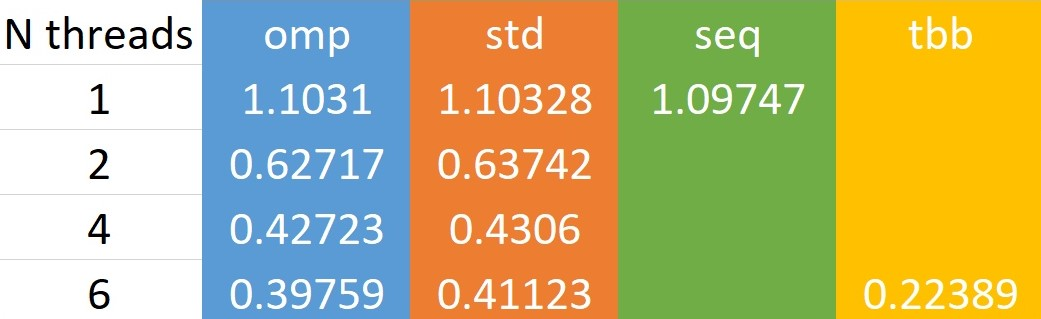
\includegraphics[width=\linewidth]{../../../../modules/reports/kornev_n_qs/result.jpg}
\caption{Результаты}
\label{ris:image}
\end{figure}

\par OpenMP и std::threads на одном потоке работают, за исключением небольшой доли погрешности, примерно за такое же время, как и последовательный алгоритм. Также приблизительное равенство сохраняется и на другом числе потоков, но, возможно стоит отметить, что std::threads немного проигрывает OpenMP на 1-2\% по времени. Трудно сказать, закономерность ли это в силу особенностей технологий или погрешность вычислений. Далее можно заметить, что увеличение числа потоков выше 4 не дает существенного прироста производительности, потому что слияние отсортированных частей происходит не на всех выделенных потоках, а лишь малым числом из них. 
\par Важно отметить, что программа с использованием TBB работает почти в 2 раза (1.8) 
быстрее OpenMP и std::threads, что объясняется наличием планировщика задач, который эффективно распределяет задачи между свободными потоками, тем самым позволяя значительно сократить время простоя процессора.  
 
\newpage
% Конец результатов экспериментов

% Заключение
\section*{Заключение}
\addcontentsline{toc}{section}{Заключение}

Выполнены следующие задачи:

\begin{enumerate} 
\item Написан последовательный алгоритм быстрой сортировки и автоматические тесты для него.
\item Написан параллельный алгоритм быстрой сортировки с простым слиянием, для возможности его реализации при помощи технологий параллельного программирования.
\item Реализован алгоритм с  использованием OpenMP, и автоматические тесты для него.
\item Реализован алгоритм с  использованием TBB, и автоматические тесты для него.
\item Реализован алгоритм с  использованием std::threads, и автоматические тесты для него.
\item Проведены вычислительные эксперименты, выполнен анализ полученных результатов. 
\end{enumerate} 

\newpage
% Конец заключения

% Список литературы
\begin{thebibliography}{1}
\addcontentsline{toc}{section}{Список литературы}

\bibitem{Gergel} Гергель В.П., Стронгин Р.Г. Основы параллельных вычислений для многопроцессорных вычислительных систем. Учебное пособие – Нижний Новгород: Изд-во ННГУ им. Н.И. Лобачевского, 2003. 184 с. ISBN 5-85746-602-4. 

\bibitem{Wiki1} Wikipedia: the free encyclopedia [Электронный ресурс] // URL: https://en.wikipedia.org/wiki/\verb|Быстрая_сортировка| (дата обращения: 20.03.2020)

\end{thebibliography}
\newpage
% Конец списка литературы

% Приложение
\section*{Приложение}
\addcontentsline{toc}{section}{Приложение}
Код:

\lstinputlisting[language=C++]{../../../../modules/task_1/kornev_n_qs/qs.h}
\lstinputlisting[language=C++]{../../../../modules/task_1/kornev_n_qs/qs.cpp}
\lstinputlisting[language=C++]{../../../../modules/task_1/kornev_n_qs/main.cpp}

\lstinputlisting[language=C++]{../../../../modules/task_2/kornev_n_qs/qs.h}
\lstinputlisting[language=C++]{../../../../modules/task_2/kornev_n_qs/qs.cpp}
\lstinputlisting[language=C++]{../../../../modules/task_2/kornev_n_qs/main.cpp}

\lstinputlisting[language=C++]{../../../../modules/task_3/kornev_n_qs/qs.h}
\lstinputlisting[language=C++]{../../../../modules/task_3/kornev_n_qs/qs.cpp}
\lstinputlisting[language=C++]{../../../../modules/task_3/kornev_n_qs/main.cpp}

\lstinputlisting[language=C++]{../../../../modules/task_4/kornev_n_qs/qs.h}
\lstinputlisting[language=C++]{../../../../modules/task_4/kornev_n_qs/qs.cpp}
\lstinputlisting[language=C++]{../../../../modules/task_4/kornev_n_qs/main.cpp}

\end{document}